%----------------------------------------------------------------------------------------
%	PACKAGES AND THEMES
%----------------------------------------------------------------------------------------
\documentclass[aspectratio=169,xcolor=dvipsnames]{beamer}
\usetheme{SimplePlus}

\usepackage[MeX]{polski}
\usepackage{hyperref}
\usepackage{graphicx} % Allows including images
\usepackage{booktabs} % Allows the use of \toprule, \midrule and \bottomrule in tables

%----------------------------------------------------------------------------------------
%	TITLE PAGE
%----------------------------------------------------------------------------------------

\title[short title]{Całki}
\subtitle{Nie takie straszne jak się wydaje}

\author{Szymon Milczek}

\date{\today} % Date, can be changed to a custom date


%----------------------------------------------------------------------------------------
%	PRESENTATION SLIDES
%----------------------------------------------------------------------------------------

\begin{document}

\begin{frame}
    % Print the title page as the first slide
    \titlepage
\end{frame}

\begin{frame}{Overview}
    \tableofcontents
\end{frame}

%------------------------------------------------
\section{Jak to ugryźć}
%------------------------------------------------

\begin{frame}{Przede wszystkim: \textbf{dużo ćwiczyć}}
    Z pewnością widzieliście ludzi którzy widzą całkę i od razu wiedzą w jaki sposób należy ją rozwiązywać. Mają oni parę sekretów:
    \begin{itemize}
        \item Ćwiczą
        \item Ćwiczą
        \item I ćwiczą
    \end{itemize}
    Niestety ale aby wyrobić sobie tę intuicję trzeba po prostu rozwiązać przynajmniej 100-200 całek. Nie ma geniuszy, którzy pierwszy raz w życiu całkę na oczy widząc od razu magicznie wiedzą co robić. To przychodzi z praktyką.
\end{frame}

%------------------------------------------------

\begin{frame}{Sposoby}
    To nie oznacza jednak że nie można sobie nieco ułatwić procesu. Najprostsze całki (czyli te, które nas interesują na tym poziomie) będą zazwyczaj rozwiązywalne tymi sposobami:

    \begin{block}{Przez podstawienie}
        Te całki zazwyczaj zawierają jakąś funkcję złożoną, pomnożoną przez coś co wygląda jak pochodna funkcji wewnętrznej. Np $e^{x^2}\cdot 2x$
    \end{block}

    \begin{block}{Przez coś tam}
        Te również zawierają jakieś dwie pomnożone przez siebie funkcje, ale żadna z nich nie jest pochodną jakiejkolwiek funkcji wewnętrznej. Np $e^x \cdot x$
    \end{block}
    
    \begin{alertblock}{Uwaga!}
        Czasem całki mogą wyglądać na łatwe do rozwiązania, w rzeczywistości będąc niemożliwe. Przykładem jest $e^{x^2}$. Różni się od $e^{x^2}\cdot 2x$ tym, że nie ma dobrego podstawienia.
    \end{alertblock}

\end{frame}

\begin{frame}{Parę przykładów}
    \begin{table}
        \begin{tabular}{c | c}
            \toprule
            \textbf{Przez podstawienie} & \textbf{Ten drugi sposób} \\
            \midrule
            $\int x e^{x^2}dx$ & $\int x e^xdx$              \\
            $\int (3x^2 + 4x)ln(x^3 + 2x^2)dx$ & $\int ln(x)dx$             \\      
            \bottomrule
        \end{tabular}
        \caption{\label{tab:całki}Całki}
    \end{table}
\end{frame}

%------------------------------------------------
\section{Wynalazcy całek}
%------------------------------------------------

\begin{frame}{Wynalazcy całek - Isaac Newton}
    \begin{columns}[c]

        \column{.45\textwidth} % Left column and width
        \textbf{Isaac Newton}\\
        Może się to wydawać zaskakujące, jeżeli ktoś zna to nazwisko jedynie z lekcji fizyki, jako należące do człowieka, który \textit{wynalazł grawitację}, lecz jego zasługi nie ograniczają się jedynie do tej dziedziny.

        \column{.5\textwidth} % Right column and width
        \begin{figure}
            \centering
            \includegraphics[width=0.5\textwidth]{newton.png}
            \caption{\label{fig:Newton}Isaac Newton}
        \end{figure}

    \end{columns}
\end{frame}


\begin{frame}{Wynalazcy całek - Gottfried Leibniz}
    \begin{columns}[c]

        \column{.5\textwidth} % Right column and width
        \begin{figure}
            \centering
            \includegraphics[width=0.5\textwidth]{leibniz.png}
            \caption{\label{fig:Leibniz}Gottfried Leibniz}
        \end{figure}
        
        \column{.45\textwidth} % Left column and width
        \textbf{Gottfried Leibniz}\\
        Mniej więcej w tym samym czasie co Newton (a nawet nieco wcześniej) odpowiedni aparat matematyczny do rozwiązywania całek opracował Gottfried Leibniz. To jemu zawdzięczamy np. używany do dziś znak $\int$ zapisywany przed każdą całką.

    \end{columns}
\end{frame}

%------------------------------------------------


%------------------------------------------------

\begin{frame}{Całki są super}
    \begin{columns}[c]
    
        \column{.45\textwidth} % Left column and width
        Powody aby nauczyć się całkować:
        \begin{enumerate}
            \item Czujesz się mądrze
            \item Podwyższony testosteron
            \item Poszerzone horyzonty
        \end{enumerate}

        \column{.5\textwidth} % Right column and width
        \begin{figure}
            \centering
            
\includegraphics[width=0.5\textwidth]{cool.png}
            \caption{\label{fig:cool}Autorski}
        \end{figure}

    \end{columns}
\end{frame}

%------------------------------------------------
\section{Całki Oznaczone}
%------------------------------------------------

\begin{frame}{Całki oznaczone}
    \begin{columns}[c]
        
        \column{.5\textwidth} % Right column and width
        \begin{figure}
            \centering
            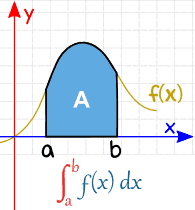
\includegraphics[width=0.5\textwidth]{oznaczone.png}
            \caption{\label{fig:oznaczone}Wizualna reprezentacja}
        \end{figure}
        
        \column{.45\textwidth} % Left column and width
        \textbf{Całka oznaczona}\\
        Całka oznaczona może być rozumiana jako funkcja zwracająca pole pod wykresem od $a$ do $b$.

    \end{columns}
\end{frame}

%------------------------------------------------

%------------------------------------------------

\begin{frame}{References}
    \begin{columns}
    
        \column{.45\textwidth}
        \footnotesize{
            \begin{thebibliography}{99}
                \bibitem[Milczek, 2022]{p1} Szymon Milczek (2022)
                \newblock Jakiś tytuł
                \newblock \emph{Dziennik} 12(3), 45 -- 678.
                \bibitem[Szymon, 2022]{p1} Szymon Milczek (2022)
                \newblock Jakiś tytuł
                \newblock \emph{Dzienniczek} 12(3), 2 -- 200.
            \end{thebibliography}
        }
        
        \column{.5\textwidth}
        \begin{figure}
            \centering
            
\includegraphics[width=0.8\textwidth]{ref.png}
        \end{figure}
    \end{columns}
\end{frame}

%-------------------------------------------------

\end{document}